%Capítulo 3

\chapter{Recurción y condicionales}

El tema principal de este capítulo es la declaración if, que ejecuta código diferente dependiendo del estado del programa. Pero primero quiero introducir dos nuevos operadores: división entera y módulo.

\section{División entera y módulo}

El operador de \textbf{división entera}, \texttt{//}, divide dos números y redondea hacia abajo a un entero. Por ejemplo, supongamos que la duración de una película es de 105 minutos. Podrías querer saber cuánto tiempo es eso en horas. La división convencional devuelve un número de punto flotante:

\begin{lstlisting}
>>> minutes = 105
>>> minutes / 60
1.75
\end{lstlisting}

Pero normalmente no escribimos las horas con puntos decimales. La división entera devuelve el número entero de horas, redondeando hacia abajo:

\begin{lstlisting}
>>> minutes = 105
>>> hours = minutes // 60
>>> hours
1
\end{lstlisting}

Para obtener el resto, podrías restar una hora en minutos:

\begin{lstlisting}
>>> remainder = minutes - hours * 60
>>> remainder
45
\end{lstlisting}

Una alternativa es usar el \textbf{operador módulo}, \texttt{\%}, que divide dos números y devuelve el resto.

\begin{lstlisting}
>>> remainder = minutes % 60
>>> remainder
45
\end{lstlisting}

El operador módulo es más útil de lo que parece. Por ejemplo, puedes verificar si un número es divisible por otro---si \texttt{x \% y} es cero, entonces $x$ es divisible por $y$.

Además, puedes extraer el código o dígitos más a la derecha de un número. Por ejemplo, \texttt{x \% 10} da como resultado el dígito más a la derecha de \texttt{x} (en base 10). De manera similar, \texttt{x \% 100} da como resultado los últimos dos dígitos.

Si estás usando Python 2, la división  funciona de manera diferente. El operador de división de punto flotante si cualqueira de los operadores es un flotante.

\section{Expresiones booleanas}

Una expresión booleana es una expresión que es verdadera o falsa. Los siguientes ejemplos usan el operador \texttt{==}, que compara dos operandos y produce \texttt{True} si son iguales y \texttt{False} en caso contrario:

\begin{lstlisting}
>>> 5 == 5
True
>>> 5 == 6
False
\end{lstlisting}

\texttt{True} y \texttt{False} son valores especiales que pertenecen al tipo \texttt{bool}; no son cadenas:

\begin{lstlisting}
>>> type(True)
<class 'bool'>
>>> type(False)
<class 'bool'>
\end{lstlisting}

El operador \texttt{==} es uno de los operadores relacionales; los otros son:

\begin{lstlisting}
x != y    # x no es igual a y
x > y     # x es mayor que y
x < y     # x es menor que y
x >= y    # x es mayor o igual que y
x <= y    # x es menor o igual que y
\end{lstlisting}

Aunque estas operaciones probablemente te resulten familiares, los símbolos de Python son diferentes de los símbolos matemáticos. Un error común es usar un solo signo igual (\texttt{=}) en lugar de un doble signo igual (\texttt{==}). Recuerda que \texttt{=} es un operador de asignación y \texttt{==} es un operador relacional. No existe tal cosa como \texttt{=<} o \texttt{=>}.

\section{Operadores lógicos}

Hay tres operadores lógicos: \texttt{and}, \texttt{or}, y \texttt{not}. La semántica (significado) de estos operadores es similar a su significado en inglés. Por ejemplo, \texttt{x > 0 and x < 10} es verdadero solo si $x$ es mayor que 0 y menor que 10.

\texttt{n\%2 == 0 or n\%3 == 0} es verdadero si cualquiera de las condiciones o ambas son verdaderas, es decir, si el número es divisible por \texttt{2 or 3}.

Finalmente, el operador \texttt{not} niega una expresión booleana, así que \texttt{not (x > y)} es verdadero si \texttt{x > y} es falso, es decir, si $x$ es menor o igual que $y$.

Estrictamente hablando, los operandos de los operadores lógicos deberían ser expresiones booleanas, pero Python no es muy estricto. Cualquier número diferente de cero se interpreta como \texttt{True}.

\begin{lstlisting}
    >>> 42 and True
    True
\end{lstlisting}

Esta flexibilidad ouede ser útil, pero hay algunas sutilezas que podrían resultar confusas. Podrías querer evitarlo (a menos que sepas lo que estás haciendo).

\section{Ejecición condicional}
para esribir programas útiles, casi siempre necesitamos la capcacidad de verificar condiciones y cambiar el comportamiento del progrema en consecuencia. Las \textbf{sentencias condicionales} nos dan esta habilidad. La forma más simple es la sentencia \texttt{if}:

\begin{lstlisting}
    if x > 0:
        print('x es positivo')
\end{lstlisting}

La expresión booleana después de \texttt{if} se llama la condición. Si es verdadera, se ejecuta la instrucción indentada. Si no, no sucede nada.

Las declaraciones \texttt{if} tienen la misma estructura que las definiciones de funciones: un encabezado seuido de un cuerpo indentado. Declaraciones como esta sellaman declaraciones cmpuestas.

No hay límite en el número de declaraciones que pueden aparecer en el cuerpo, ero debe habero al menos una. Ocasionalmente, es útil tener un cuerpo sin declaraciones (generalmente como un marcador de posicion para el código no escrito aún). En ese caso, puedes usar la declaración \texttt{pass}, que no hace nada.

\begin{lstlisting}
    if x < 0:
        pass    #TODO: necesito manejar los valores negativos
\end{lstlisting}

\section{Ejecución alternativa}

Una segunda forma de la declaraión \texttt{if} es la "ejecición alternativa" , en la que hay dos posibilidades y la condición determina cuál se ejecuta. La sinaxis es la siguiente:

\begin{lstlisting}
    if x % 2 == 0:
        print('x es par')
    else:
        print('x es impar')
\end{lstlisting}

Si el resto cuando x se divide por 2 es 0, entoncessabemos que x es par, y el programa muestra un mensaje apropiado. Si la condición es falsa, se ejecuta el segundo conjunto de instrucciones. Dado que la condición debe ser verdadera o falsa, exactamente una de las alternativas se ejecutará. Las alternativas se llaman ramas, porque son ramas en el flujo de ejecición.

\section{Condicionales unidas}

A veces hay más de dos posibilidades y necesitamos más de dos ramas. Una forma de expresar un cálculo así es una condicional encadenada:

\begin{lstlisting}
    if x < y:
        print('x es menor que y')
    elif x > y:
        print('x es mayor que y')
    else:
        print('x es igual a y')
\end{lstlisting}

\texttt{elif} es una abreviatura de "else if". Nuevamente, exactamente una rama se ejecutará. No hay límite en el número de declaraciones \texttt{elif}. SI hay un cláusula \texttt{else}, tiene que estar al final, pero no es necesario que haya una.

\begin{lstlisting}
    if choice == 'a':
        draw_a()
    elif choice == 'b':
        draw_n()
    elif choice == 'c':
        draw_c()
\end{lstlisting}

Cada condición se verifica en orden. Si la primera es falsa, se verifica la siguiente, y así sucesivamente. Si una de ellas es verdadera, se ejecuta la rama correspondiente y la declaración termina. Incluso si más de una condición es verdadera, solo se ejecuta la primera rama verdadera.

\section{Condicionales anidadas}

Una condicional también puede estar anidada dentro de otra. Podríamos haber escrito el ejemplo de la sección anterior de esta manera:

\begin{lstlisting}
if x == y:
    print('x y y son iguales')
else:
    if x < y:
        print('x es menor que y')
    else:
        print('x es mayor que y')
\end{lstlisting}

La condicional externa contiene dos ramas. La primera rama contiene una declaración simple. La segunda rama contiene otra declaración \texttt{if}, que tiene dos ramas propias. Esas dos ramas son ambas declaraciones simples, aunque también podrían haber sido declaraciones condicionales.

Aunque la indentación de las declaraciones hace que la estructura sea evidente, las condicionales anidadas se vuelven difíciles de leer muy rápidamente. Es una buena idea evitarlas cuando sea posible.

Los operadores lógicos a menudo proporcionan una manera de simplificar las declaraciones condicionales anidadas. Por ejemplo, podemos reescribir el siguiente código usando una sola condicional:

\begin{lstlisting}
if 0 < x:
    if x < 10:
        print('x is a positive single-digit number.')
\end{lstlisting}

La declaración \texttt{print} se ejecuta solo si pasamos ambas condicionales, así que podemos obtener el mismo efecto con el operador \texttt{and}:

\begin{lstlisting}
if 0 < x and x < 10:
    print('x es un numero positivo de un solo digito.')
\end{lstlisting}

Para ese tipo de condición, Python proporciona una opción más concisa:

\begin{lstlisting}
def coundown(n):
if 0 < x < 10:
    print('x es un numero positivo de un solo digito.')
\end{lstlisting}

\section{Recursión}

Es legal que una función llame a otra; también es legal que una función se llame a sí misma. Puede que no sea obvio por qué eso es algo bueno, pero resulta ser una de las cosas más mágicas que un programa puede hacer. Por ejemplo, observa la siguiente función:

\begin{lstlisting}
def countdown(n):
    if n <= 0:
        print('Despegue!')
    else:
        print(n)
        countdown(n - 1)
\end{lstlisting}

Si \texttt{n} es 0 o negativo, devuelve la palabra "Despegue". De lo contrario, devuelve \texttt{n} y luego llama a la función \texttt{countdown} \_\_itself\_\_ pasando \texttt{n - 1} como argumento.

¿Qué pasa si llamamos a esta función así?

\begin{lstlisting}
>>> countdown(3)
\end{lstlisting}

La ejecución de \texttt{countdown} comienza con $n=3$, y como $n$ es mayor que 0, imprime el valor 3, y luego se llama a sí misma...

\quad La ejecución de \texttt{countdown} comienza con $n=2$, y como $n$ es mayor que 0, imprime el valor 2, y luego se llama a sí misma...

\quad\quad La ejecución de \texttt{countdown} comienza con $n=1$, y como $n$ es mayor que 0, imprime el valor 1, y luego se llama a sí misma...

\quad\quad\quad La ejecución de \texttt{countdown} comienza con $n=0$, y como $n$ no es mayor que 0, imprime la palabra ``Blastoff!'' y luego regresa.

\quad\quad El \texttt{countdown} que recibió $n=1$ regresa.

\quad El \texttt{countdown} que recibió $n=2$ regresa.

El \texttt{countdown} que recibió $n=3$ regresa.

Y entonces estás de vuelta en \texttt{\_\_main\_\_}. Así, la salida total se ve así:

\begin{lstlisting}
3
2
1
Despegue!
\end{lstlisting}

Una función que se llama a sí misma es recursiva; el proceso de ejecutarla se llama recursión.

Como otro ejemplo, podemos escribir una función que imprima una cadena $n$ veces.

\begin{lstlisting}
def print_n(s, n):
    if n <= 0:
        return
    print(s)
    print_n(s, n-1)
\end{lstlisting}

\begin{figure}[h]
\centering
\begin{tabular}{|c|c|}
\hline
\texttt{\_\_main\_\_} & \phantom{n $\rightarrow$ 3} \\
\hline
\texttt{countdown} & n $\rightarrow$ 3 \\
\hline
\texttt{countdown} & n $\rightarrow$ 2 \\
\hline
\texttt{countdown} & n $\rightarrow$ 1 \\
\hline
\texttt{countdown} & n $\rightarrow$ 0 \\
\hline
\end{tabular}
\caption{Diagrama de pila.}
\label{fig:diagrama_de_pila}
\end{figure}

Si \texttt{n <= 0} la \textbf{declaración return} sale de la función. El flujo de ejecución inmediatamente regresa al llamador, y las líneas restantes de la función no se ejecutan.

El resto de la función es similar a \texttt{countdown}: muestra \texttt{s} y luego se llama a sí misma para mostrar \texttt{s} $n-1$ veces adicionales. Así que el número de líneas de salida es $1 + (n-1)$, que suma $n$.

Para ejemplos simples como este, es probablemente más fácil usar un bucle \texttt{for}. Pero veremos ejemplos más adelante que son difíciles de escribir con un bucle \texttt{for} y fáciles de escribir con recursión, así que es bueno empezar temprano.

\section{Diagramas de pila para funciones recursivas}

En la Sección~\ref{sec:diagramas_de_pila} usamos un diagrama de pila para representar el estado de un programa durante una llamada a función. El mismo tipo de diagrama puede ayudar a interpretar una función recursiva.

Cada vez que se llama a una función, Python crea un marco para contener las variables locales y parámetros de la función. Para una función recursiva, podría haber más de un marco en la pila al mismo tiempo.

La Figura~\ref{fig:diagrama_de_pila} muestra un diagrama de pila para \texttt{countdown} llamada con $n = 3$.

Como de costumbre, la parte superior de la pila es el marco para \texttt{\_\_main\_\_}. Está vacío porque no creamos ninguna variable en \texttt{\_\_main\_\_} ni le pasamos argumentos.

Los cuatro marcos de \texttt{countdown} tienen diferentes valores para el parámetro $n$. La parte inferior de la pila, donde $n=0$, se llama el \textbf{caso base}. No hace una llamada recursiva, así que no hay más marcos.

Como ejercicio, dibuja un diagrama de pila para \texttt{print\_n} llamada con $s = $ `Hello' y $n=2$. Luego escribe una función llamada \texttt{do\_n} que tome un objeto función y un número, $n$, como argumentos, y que llame a la función dada $n$ veces.

Una función que se llama a sí misma es recursiva; el proceso de ejecutarla se llama recursión.

Como otro ejemplo, podemos escribir una función que imprima una cadena $n$ veces.

\section{Recursión infinita}

Si una recursión nunca alcanza un caso base, continúa haciendo llamadas recursivas para siempre, y el programa nunca termina. Esto se conoce como \textbf{recursión infinita}, y generalmente no es una buena idea. Aquí hay un programa mínimo con recursión infinita:

\begin{lstlisting}
def recursion():
    recursion()
\end{lstlisting}

En la mayoría de entornos de programación, un programa con recursión infinita no se ejecuta realmente para siempre. Python reporta un mensaje de error cuando se alcanza la profundidad máxima de recursión:

\begin{lstlisting}
File "<stdin>", line 2, in recurse
File "<stdin>", line 2, in recurse
File "<stdin>", line 2, in recurse
                    .
                    .
                    .
File "<stdin>", line 2, in recurse
RuntimeError: Maximum recursion depth exceeded
\end{lstlisting}

Este traceback es un poco más grande que el que vimos en el capítulo anterior. Cuando ocurre el error, ¡hay 1000 marcos de \texttt{recurse} en la pila!

Si encuentras una recursión infinita por accidente, revisa tu función para confirmar que hay un caso base que no hace una llamada recursiva. Y si hay un caso base, verifica si tienes garantía de alcanzarlo.

\section{Entrada de teclado}

Los programas que hemos escrito hasta ahora no aceptan entrada del usuario. Simplemente hacen lo mismo cada vez.

Python proporciona una función integrada llamada \texttt{input} que detiene el programa y espera a que el usuario escriba algo. Cuando el usuario presiona Return o Enter, el programa se reanuda e \texttt{input} devuelve lo que el usuario escribió como una cadena. En Python 2, la misma función se llama \texttt{raw\_input}.

\begin{lstlisting}
>>> text = input()
What are you waiting for?
>>> text
'What are you waiting for?'
\end{lstlisting}

Antes de obtener entrada del usuario, es buena idea imprimir un mensaje diciendo al usuario qué escribir. \texttt{input} puede tomar un mensaje como argumento:

\begin{lstlisting}
>>> nombre = input('cual es tu nombre?\n')
cual es tu nombre?
Arthur, rey de Britons!
>>> name
'Arthur, rey de Britons!'
\end{lstlisting}

La secuencia \texttt{\textbackslash n} al final del mensaje representa una \textbf{nueva línea}, que es un carácter especial que causa un salto de línea. Por eso la entrada del usuario aparece debajo del mensaje.

Si esperas que el usuario escriba un entero, puedes tratar de convertir el valor de retorno a \texttt{int}:

\begin{lstlisting}
>>> prompt = 'What...is the airspeed velocity of an unladen swallow?\n'
>>> speed = input(prompt)
What...is the airspeed velocity of an unladen swallow?
42
>>> int(speed)
42
\end{lstlisting}

Pero si el usuario escribe algo que no sea una cadena de dígitos, obtienes un error:

\begin{lstlisting}
>>> speed = input(prompt)
What...is the airspeed velocity of an unladen swallow?
What do you mean, an African or a European swallow?
>>> int(speed)
ValueError: invalid literal for int() with base 10
\end{lstlisting}

Veremos cómo manejar este tipo de error más adelante.

\section{Depuración}

Cuando ocurre un error de sintaxis o de ejecución, el mensaje de error contiene mucha información, pero puede ser abrumador. Las partes más útiles usualmente son:

\begin{itemize}
\item Qué tipo de error fue, y
\item Dónde ocurrió.
\end{itemize}

Los errores de sintaxis son usualmente fáciles de encontrar, pero hay algunas trampas. Los errores de espacios en blanco pueden ser complicados porque los espacios y tabulaciones son invisibles y estamos acostumbrados a ignorarlos.

\begin{lstlisting}
>>> x = 5
>>>  y = 6
  File "<stdin>", line 1
    y = 6
    ^
IndentationError: unexpected indent
\end{lstlisting}

En este ejemplo, el problema es que la segunda línea está indentada por un espacio. Pero el mensaje de error apunta a \texttt{y}, que es engañoso. En general, los mensajes de error indican dónde se descubrió el problema, pero el error real podría estar antes en el código, algunas veces en una línea anterior.

Lo mismo es cierto para los errores de ejecución. Supongamos que estás tratando de calcular una relación señal-ruido en decibeles. La fórmula es $SNR_{db} = 10 \log_{10}(P_{signal}/P_{noise})$. En Python, podrías escribir algo como esto:

\begin{lstlisting}
import math
signal_power = 9
noise_power = 10
ratio = signal_power // noise_power
decibels = 10 * math.log10(ratio)
print(decibels)
\end{lstlisting}

Cuando ejecutas este programa, obtienes una excepción:

\begin{lstlisting}
Traceback (most recent call last):
  File "snr.py", line 5, in ?
    decibels = 10 * math.log10(ratio)
ValueError: math domain error
\end{lstlisting}

El mensaje de error indica la línea 5, pero no hay nada malo con esa línea. Para encontrar el error real, podría ser útil imprimir el valor de \texttt{ratio}, que resulta ser 0. El problema está en la línea 4, que usa división entera en lugar de división de punto flotante.

Deberías tomarte el tiempo para leer los mensajes de error cuidadosamente, pero no asumas que todo lo que dicen es correcto.

\section{Glosario}

\textbf{división entera:} Un operador, denotado \texttt{//}, que divide dos números y redondea hacia abajo (hacia el infinito negativo) a un entero.

\textbf{operador módulo:} Un operador, denotado con un signo de porcentaje (\texttt{\%}), que funciona con enteros y devuelve el resto cuando un número es dividido por otro.

\textbf{expresión booleana:} Una expresión cuyo valor es \texttt{True} o \texttt{False}.

\textbf{operador relacional:} Uno de los operadores que compara sus operandos: \texttt{==}, \texttt{!=}, \texttt{>}, \texttt{<}, \texttt{>=}, y \texttt{<=}.

\textbf{operador lógico:} Uno de los operadores que combina expresiones booleanas: \texttt{and}, \texttt{or}, y \texttt{not}.

\textbf{declaración condicional:} Una declaración que controla el flujo de ejecución dependiendo de alguna condición.

\textbf{condición:} La expresión booleana en una declaración condicional que determina qué rama se ejecuta.

\textbf{declaración compuesta:} Una declaración que consiste de un encabezado y un cuerpo. El encabezado termina con dos puntos (:). El cuerpo está indentado relativo al encabezado.

\textbf{rama:} Una de las secuencias alternativas de declaraciones en una declaración condicional.

\textbf{condicional encadenada:} Una declaración condicional con una serie de ramas alternativas.

\textbf{condicional anidada:} Una declaración condicional que aparece en una de las ramas de otra declaración condicional.

\textbf{declaración return:} Una declaración que causa que una función termine inmediatamente y regrese al llamador.

\textbf{recursión:} El proceso de llamar a la función que se está ejecutando actualmente.

\textbf{caso base:} Una rama condicional en una función recursiva que no hace una llamada recursiva.

\textbf{recursión infinita:} Una recursión que no tiene un caso base, o nunca lo alcanza. Eventualmente, una recursión infinita causa un error de tiempo de ejecución.

\section{Ejercicios}

\textbf{Ejercicio 5.1.} El módulo \texttt{time} proporciona una función, también llamada \texttt{time}, que devuelve la Hora Media de Greenwich actual en ``la época'', que es un tiempo arbitrario usado como punto de referencia. En sistemas UNIX, la época es el 1 de enero de 1970.

\begin{lstlisting}
>>> import time
>>> time.time()
1437746094.5735958
\end{lstlisting}

Escribe un script que lea la hora actual y la convierta a una hora del día en horas, minutos y segundos, más el número de días desde la época.

\textbf{Ejercicio 5.2.} El Último Teorema de Fermat dice que no hay enteros positivos $a$, $b$, y $c$ tales que
$$a^n + b^n = c^n$$
para cualquier valor de $n$ mayor que 2.

\begin{enumerate}
\item Escribe una función llamada \texttt{check\_fermat} que tome cuatro parámetros---$a$, $b$, $c$ y $n$---y verifique si se cumple el teorema de Fermat. Si $n$ es mayor que 2 y
$$a^n + b^n = c^n$$
el programa debe imprimir, ``¡Santo cielo, Fermat estaba equivocado!'' De lo contrario, el programa debe imprimir, ``No, eso no funciona.''

\item Escribe una función que solicite al usuario ingresar valores para $a$, $b$, $c$ y $n$, los convierta a enteros, y use \texttt{check\_fermat} para verificar si violan el teorema de Fermat.
\end{enumerate}

\textbf{Ejercicio 5.3.} Si te dan tres palos, puedes o no ser capaz de organizarlos en un triángulo. Por ejemplo, si uno de los palos tiene 12 pulgadas de largo y los otros dos tienen una pulgada de largo, no podrás hacer que los palos cortos se encuentren en el medio. Para cualquier longitud, hay una prueba simple para ver si es posible formar un triángulo:

\emph{Si cualquiera de las tres longitudes es mayor que la suma de las otras dos, entonces no puedes formar un triángulo. De lo contrario, puedes. (Si la suma de dos longitudes es igual a la tercera, forman lo que se llama un triángulo ``degenerado''.)}

\begin{enumerate}
\item Escribe una función llamada \texttt{is\_triangle} que tome tres enteros como argumentos, y que imprima ``Sí'' o ``No'', dependiendo de si puedes o no formar un triángulo a partir de palos con las longitudes dadas.

\item Escribe una función que solicite al usuario ingresar tres longitudes de palos, las convierta a enteros, y use \texttt{is\_triangle} para verificar si los palos con las longitudes dadas pueden formar un triángulo.
\end{enumerate}

\textbf{Ejercicio 5.4.} ¿Cuál es la salida del siguiente programa? Dibuja un diagrama de pila que muestre el estado del programa cuando imprime el resultado.

\begin{lstlisting}
def recurse(n, s):
    if n == 0:
        print(s)
    else:
        recurse(n-1, n+s)

recurse(3, 0)
\end{lstlisting}

\begin{enumerate}
\item ¿Qué pasaría si llamaras a esta función así: \texttt{recurse(-1, 0)}?

\item Escribe una docstring que explique todo lo que alguien necesitaría saber para usar esta función (y nada más).
\end{enumerate}

Los siguientes ejercicios usan el módulo \texttt{turtle}, descrito en el Capítulo 4

\textbf{Ejercicio 5.5.} Lee la siguiente función y ve si puedes descifrar qué hace (ver los ejemplos en el Capítulo 4). Luego ejecútala y ve si la entendiste bien.

\begin{figure}[h]
\centering
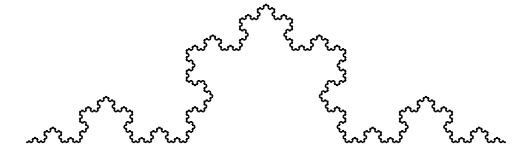
\includegraphics[width=0.7\linewidth]{images/chapter_5_2.png} % Ajusta el nombre del archivo
\caption{Una curva de Koch.}
\label{fig:koch}
\end{figure}


\begin{lstlisting}
def draw(t, length, n):
    if n == 0:
        return
    angle = 50
    t.fd(length*n)
    t.lt(angle)
    draw(t, length, n-1)
    t.rt(2*angle)
    draw(t, length, n-1)
    t.lt(angle)
    t.bk(length*n)
\end{lstlisting}

\textbf{Ejercicio 5.6.} La curva de Koch es un fractal que se parece algo a la Figura~\ref{fig:koch}. Para dibujar una curva de Koch con longitud $x$, todo lo que tienes que hacer es

\begin{enumerate}
\item Dibujar una curva de Koch con longitud $x/3$.
\item Girar a la izquierda 60 grados.
\item Dibujar una curva de Koch con longitud $x/3$.
\item Girar a la derecha 120 grados.
\item Dibujar una curva de Koch con longitud $x/3$.
\item Girar a la izquierda 60 grados.
\item Dibujar una curva de Koch con longitud $x/3$.
\end{enumerate}

La excepción es si $x$ es menor que 3: en ese caso, puedes simplemente dibujar una línea recta con longitud $x$.

\begin{enumerate}
\item Escribe una función llamada \texttt{koch} que tome una tortuga y una longitud como parámetros, y que use la tortuga para dibujar una curva de Koch con la longitud dada.

\item Escribe una función llamada \texttt{snowflake} que dibuje tres curvas de Koch para hacer el contorno de un copo de nieve.

Solución: \texttt{https://thinkpython.com/code/koch.py}

\item La curva de Koch puede generalizarse de varias maneras. Ve \texttt{http://en.wikipedia.org/wiki/Koch\_snowflake} para ejemplos e implementa tu fractal favorito.
\end{enumerate}
